% arXiv preprint — Quantum journal style (quantumarticle.cls)
% Compile with pdfLaTeX (twice for cross-references).
\documentclass[aps,a4paper,onecolumn,11pt,unpublished]{quantumarticle}
\pdfoutput=1

\usepackage{amsmath,amssymb}
\usepackage{booktabs}
\usepackage{graphicx}
\usepackage{xcolor}
% quantumarticle loads hyperref at \begin{document}; loading it here avoids
% the late nameref hook-rule error in recent LaTeX kernels.
\usepackage{xurl}
\usepackage{hyperref}
\setlength{\emergencystretch}{2em}

\newcommand{\dF}{\Delta\mathrm{F1}}
\newcommand{\dA}{\Delta\mathrm{ACC}}
\newcommand{\pp}{\,\mathrm{pp}}

\begin{document}

\title{HyQ-LC: Improving Light-Curve Classification with Hybrid Quantum--Classical Learning}

\author[orcid=0009-0000-4773-6574]{Xinghang Yu}
\email{3023244355@tju.edu.cn}
\affiliation{School of Computer Science and Technology, Tianjin University, 135 Yaguan Road, Haihe Education Park, Tianjin 300350, People's Republic of China}
\author[orcid=0000-0002-3783-2228]{Bin Yang}
\affiliation{School of Computer Science and Technology, Tianjin University, 135 Yaguan Road, Haihe Education Park, Tianjin 300350, People's Republic of China}
\email{yangbincic@tju.edu.cn}

\begin{abstract}
Light curves trace stellar variability and support studies of stellar evolution and cosmic distances. Large time-domain surveys therefore require reliable, scalable methods for classifying variable stars. Classical feature-based models provide a practical approach, while variational quantum circuits offer a complementary representation through quantum-state encoding and observable measurements. Here we introduce HyQ-LC, a hybrid quantum--classical classifier for ten variable-star classes using 359 handcrafted features and 633{,}034 training objects. We evaluate its performance using parameter-matched MLPs, classical branch replacements, and an approximately leaf-budget-matched LightGBM control. On a 20{,}000-object test set, the 44{,}238-parameter hybrid achieves higher Macro-F1 than a strictly parameter-matched MLP, with gains of 0.8276 and 1.2393 percentage points on two audited seeds. On the same test objects, a separate 55{,}581-parameter fixed-fusion configuration achieves slightly higher Macro-F1 but lower accuracy than approximately budget-matched LightGBM, with the main positive class-level differences in CEP, RRC, and ROT. Full-budget LightGBM remains stronger overall. All comparisons use frozen data splits, validation-only model selection, and independently audited per-object predictions. Data, code, and comparison records are available at \url{https://github.com/bestdo77/quantum-lightcurve-hybrid}. These results support the empirical value of the tested hybrid representations under specified comparison conditions.
\end{abstract}

\maketitle

\section{Introduction}

Large sky surveys require scalable methods for classifying astronomical observations~\cite{moriwaki2023}. Light-curve classification approaches range from variability features and hierarchical random forests in ALeRCE~\cite{alerce2021} to learned sequence representations in ASTROMER~\cite{astromer2023}. TDLight combines incremental light-curve management with trigger-based classification and confidence-controlled database write-back~\cite{tdlight2026}. StarEmbed benchmarks time-series foundation models against domain-specific baselines on variable-star observations~\cite{starembed2026}. Shao et al. combine light-curve measurements and physical parameters through structured sequence modelling with large language models~\cite{shao2026}. These studies use different inputs, class definitions, and evaluation protocols; their reported scores are not direct baselines for the present ten-class task.

Hybrid quantum--classical networks provide a route for combining classical representations with variational quantum circuits~\cite{mari2020}. In astronomy, Peters et al. demonstrated quantum-kernel classification of supernova spectral features on a noisy processor~\cite{peters2021}. More recently, Chen and Kuo compared fully connected, residual, and attention-based variational circuits on tabular benchmarks~\cite{chenkuo2026}. These studies motivate testing quantum representations for light-curve features, but do not establish an advantage on the present data.

Benchmark design is central to interpreting such tests. Bowles et al. found that classical baselines generally outperformed quantum classifiers across their benchmarks, and that removing entanglement often preserved or improved performance~\cite{bowles2024}. We therefore use controlled comparisons to separate model capacity, branch design, and training exposure. This paper reports such a result for large-scale light-curve classification: \textbf{a hybrid quantum--classical model achieves higher Macro-F1 point estimates than a same-parameter pure MLP, selected classical replacement branches, and approximately budget-matched LightGBM on a shared 20{,}000-object test set, with uncertainty depending on the comparison and seed.}

We organise the paper around exactly these three findings:
\begin{enumerate}
  \item \textbf{Same-parameter pure-MLP control.} On the 20{,}000-object test set, two audited fine-tuning seeds improve Macro-F1 by $0.83$--$1.24$ percentage points over a pure MLP with the same total of 44{,}238 parameters. The seed-44 paired interval excludes zero; the seed-42 interval includes zero.
  \item \textbf{Same-architecture classical replacements.} Test-set Macro-F1 point differences favour the quantum branch on the two main seeds and the older fixed-fusion configuration, but the paired intervals include zero.
  \item \textbf{Approximately budget-matched LightGBM.} On the 20{,}000-object test set, the fixed-fusion hybrid achieves slightly higher Macro-F1 and lower accuracy than a LightGBM control with a similar scalar leaf-output budget; the positive class-level differences are concentrated in CEP, RRC, and ROT.
\end{enumerate}

The evidence is designed to be independently checkable. Model selection uses only validation objects; every reported comparison uses the same test IDs and labels and can be traced to checkpoint and prediction hashes. We release the test features, labels, per-object predictions, model code, and a portable recomputation script alongside the paper~\cite{artifacts}.

\section{Models and Controlled Comparisons}

\subsection{Task and evaluation splits}

The task is classification of survey light curves into ten variable-star classes: CEP, DSCT, EA, EW, M, Non-var, ROT, RRAB, RRC, and SR. Each object is represented by 359 preprocessed handcrafted features. The training pool contains 633{,}034 objects. All reported test metrics use the same 20{,}000 unique objects and labels. The class counts, in the order above, are 45, 337, 912, 6{,}307, 352, 2{,}566, 2{,}257, 796, 357, and 6{,}071.

The main 44{,}238-parameter models use 105{,}297 validation objects for model selection; the earlier fixed-fusion and leaf-budget LightGBM experiments use 10{,}000 validation objects. Existing checkpoints, learning rates, prior corrections, and fusion coefficients are retained without reselection on the test set. The current reporting scope was obtained by matching test IDs and labels within previously saved prediction files. The test cohort had already been examined in exploratory analyses; it is the final reported test cohort, rather than an unopened confirmation cohort. Separate sealed confirmation data remain unused.

\subsection{Hybrid architectures}

The main hybrid combines a classical window-attention backbone (M8, 23{,}170 parameters) with a 9-qubit, 12-layer angle-re-uploading readout~\cite{reuploading}. The circuit has 324 rotation parameters, 108 re-uploading frequencies, and 108 shifts, for 540 quantum parameters in total. It produces 27 single-qubit $X/Y/Z$ expectation values, using the local observables employed in projected quantum representations~\cite{huang2021}. These features and the backbone's 120-dimensional representation enter a residual fusion head; the complete model has 44{,}238 parameters. Figure~\ref{fig:arch} illustrates the hybrid pipeline.

Repeated encoding can enrich the accessible frequency spectrum~\cite{encoding2021}, but increasing depth need not improve predictive performance~\cite{wang2025}. These results motivate the encoding design and empirical controls; we do not infer a task-specific advantage from expressivity alone.

\begin{figure}[t]
\centering
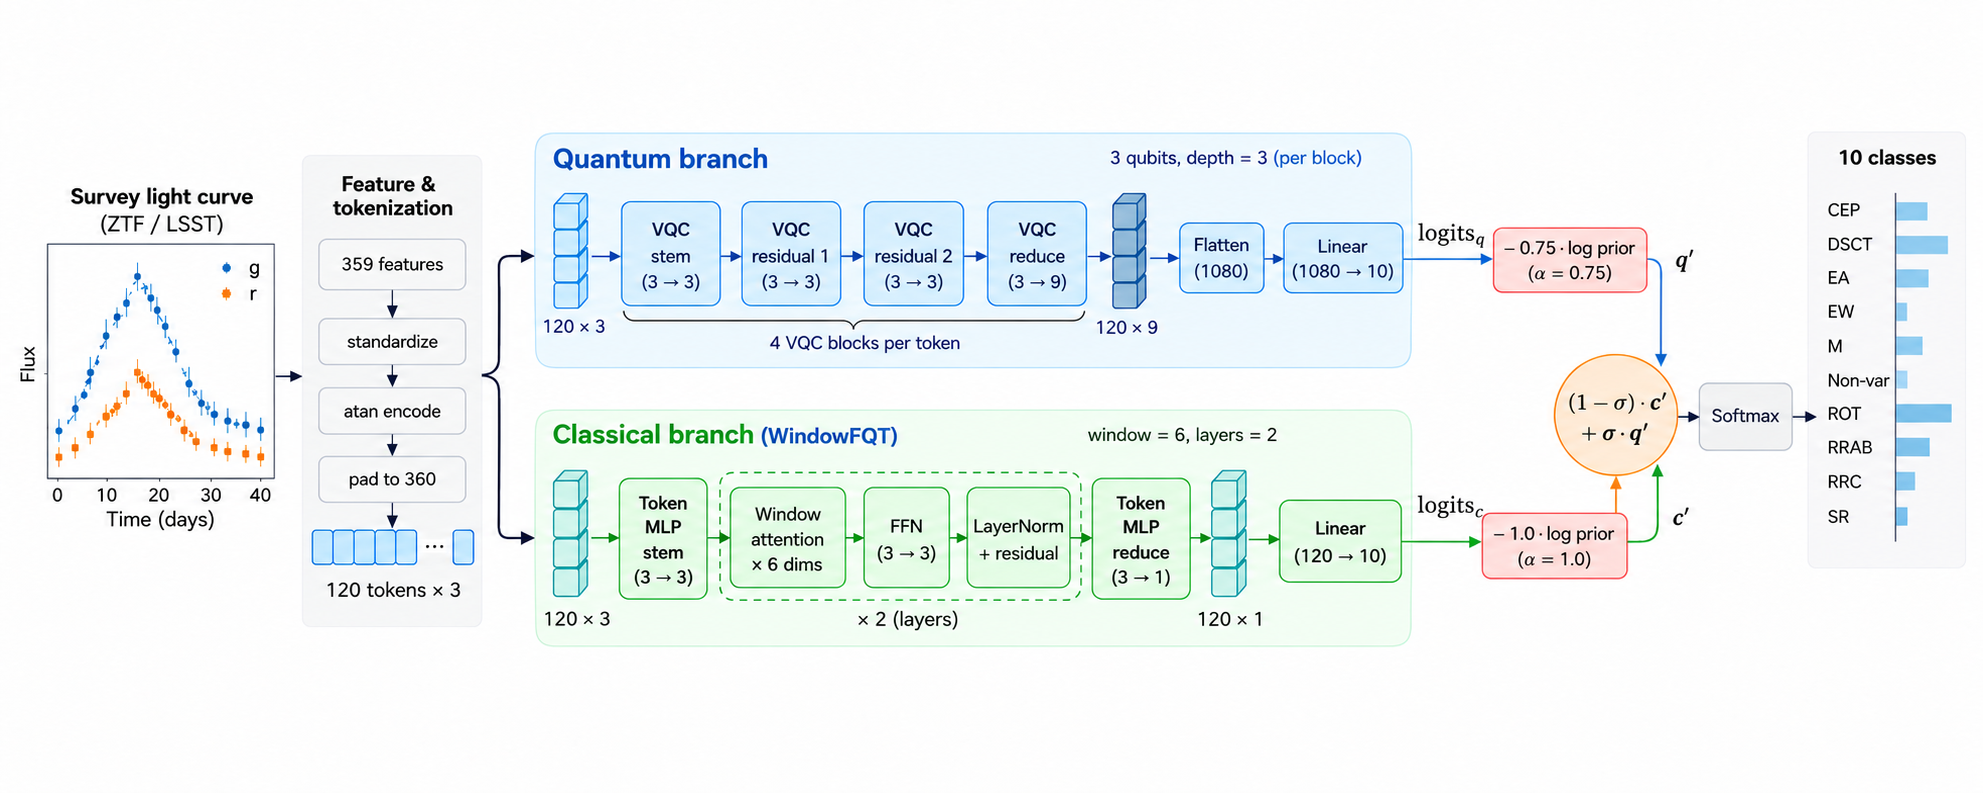
\includegraphics[width=\textwidth]{fig_architecture.png}
\caption{Hybrid quantum--classical light-curve classifier. Handcrafted features are standardised, angle-encoded, and tokenised before entering quantum and classical branches. Their representations are combined for 10-class prediction. The controlled comparisons replace only the relevant branch while preserving the shared architecture and evaluation protocol.}
\label{fig:arch}
\end{figure}

A second, older fixed-fusion configuration combines a 32{,}410-parameter token-wise quantum branch with M8 through fixed logit fusion, for 55{,}581 parameters. Its classical replacement uses MLP+MLP fusion with 54{,}631 parameters. These configurations enable direct same-architecture comparisons and the approximate LightGBM budget match described below.

\subsection{Control definitions}

\paragraph{Same-parameter pure MLP.} The pure MLP has exactly 44{,}238 parameters and is trained from scratch for 80 epochs. The hybrid uses the fixed 40-epoch M8 pre-training followed by 40 fine-tuning epochs, matching maximum object presentations. Two pre-declared learning rates are considered, with selection performed only on validation.

\paragraph{Same-architecture replacements.} In the main architecture, the quantum readout is replaced by a 540-parameter classical MLP branch while retaining the backbone, fusion-head initialisation, optimiser groups, sample order, and total parameter budget. In the older architecture, the comparison is direct: quantum+MLP fixed fusion versus MLP+MLP fixed fusion.

\paragraph{Approximately budget-matched LightGBM.} The LightGBM~\cite{lightgbm} budget is defined as the cumulative number of scalar leaf outputs across all class trees, targeting the fixed-fusion model's 55{,}581-parameter budget. The selected configuration uses 15 leaves and 370 boosting rounds (3{,}700 class trees), yielding 55{,}500 leaf values. Split-node features and thresholds are reported separately and are not included in this approximate capacity budget. This is therefore a leaf-output budget match, not an exact equivalence between tree and neural parameters.

\subsection{Selection, auditing, and uncertainty}

Checkpoints, prior-correction coefficients, and pre-declared learning rates are selected only on validation. The main comparisons use 10{,}000 paired object-level bootstrap resamples to estimate 95\% confidence intervals for metric differences. Both models use the same objects in each resample. Intervals are conditional on the fitted models; they exclude variability from training seeds and repeated model search. No multiple-comparison correction is applied. Selected checkpoints pass strict numerical audits, including independent CPU FP32 reloads; the reported test metrics are independently recomputed from ID-checked saved predictions.

\section{Results}

\subsection{Advantage over the same-parameter pure MLP}
\label{sec:sameparameter}

Table~\ref{tab:puremlp} compares the 44{,}238-parameter hybrid and pure MLP on the same 20{,}000 test objects used for the fixed-fusion comparisons below. Macro-F1 and accuracy were higher for the hybrid on both audited seeds. The seed-42 Macro-F1 interval included zero, whereas the seed-44 interval was positive; both accuracy intervals were positive. These are fixed-model, exploratory subset comparisons.

\begin{table}[t]
\centering
\caption{Same-parameter comparison on the 20{,}000-object test set. Both models have 44{,}238 parameters. Differences are hybrid minus pure MLP; intervals are based on 10{,}000 paired object-level bootstrap resamples.}
\label{tab:puremlp}
\small
\setlength{\tabcolsep}{4pt}
\begin{tabular}{@{}cccccc@{}}
\toprule
Seed & Hybrid F1 & Pure-MLP F1 & $\dF$ (pp) & 95\% interval & $\dA$ (pp) \\
\midrule
42 & 92.2913 & 91.4637 & $+0.8276$ & $[-0.0650,+1.6945]$ & $+0.6000$ $[+0.3450,+0.8550]$ \\
44 & 92.3005 & 91.0611 & $+1.2393$ & $[+0.5153,+2.0053]$ & $+0.8450$ $[+0.5900,+1.1000]$ \\
\bottomrule
\end{tabular}
\end{table}

The positive point differences on both seeds indicate a benefit under this parameter-matched comparison, with stronger interval support for seed~44. The intervals are conditional on the fitted models and do not measure variation across independent backbone pre-trainings.

\subsection{Classical branch replacement comparisons}

The branch-replacement comparison uses the same 20{,}000 test objects. On seed~44, the hybrid reached 92.3005\% Macro-F1 versus 92.0039\% for the same-parameter classical MLP replacement. Seed~42 also had a small positive F1 point difference. The fixed-fusion model reached 92.3371\% versus 92.1510\% for the classical MLP+MLP fusion. All three paired F1 intervals include zero (Table~\ref{tab:replacements}), so these comparisons indicate possible complementarity without a statistically resolved branch advantage on this test cohort.

\begin{table}[t]
\centering
\footnotesize
\setlength{\tabcolsep}{3.5pt}
\caption{Classical replacement comparisons on the same 20{,}000-object test set. Parameter counts are quantum/classical; all intervals are paired object-bootstrap 95\% intervals.}
\label{tab:replacements}
\begin{tabular}{@{}llll@{}}
\toprule
Control & Parameters (Q/C) & Seed & $\dF$ (pp), 95\% interval \\
\midrule
MLP replacement & 44{,}238/44{,}238 & 42 & $+0.0205$ $[-0.3299,+0.3726]$ \\
MLP replacement & 44{,}238/44{,}238 & 44 & $+0.2965$ $[-0.0333,+0.6982]$ \\
MLP+MLP fusion & 55{,}581/54{,}631 & 42 & $+0.1860$ $[-0.2869,+0.6740]$ \\
\bottomrule
\end{tabular}
\end{table}

\subsection{LightGBM comparison on the test set}

Table~\ref{tab:leafbudget} compares the 55{,}581-parameter fixed-fusion hybrid with the 55{,}500-leaf-value LightGBM. On the 20{,}000-object test set, the hybrid achieved slightly higher Macro-F1 (92.3371\% versus 92.2204\%; $+0.1166\pp$) but lower accuracy (94.7450\% versus 94.8650\%; $-0.1200\pp$), corresponding to 24 fewer correct predictions. The largest positive class-level F1 differences were in CEP ($+1.0040\pp$, 45 objects), RRC ($+1.1429\pp$, 357 objects), and ROT ($+0.5128\pp$, 2{,}257 objects). CEP and RRC are among the smaller classes in this set; their contributions receive equal class weight in Macro-F1 despite their small object counts. These exploratory class-level differences describe where the gain occurred and do not establish a general improvement across minority classes.

The same fixed-fusion hybrid also achieved higher test-set Macro-F1 than the 54{,}631-parameter MLP+MLP fusion (92.1510\%), with nearly identical accuracy (94.7500\%). This is an approximate parameter-budget comparison. The strictly parameter-matched pure-MLP comparison in Section~\ref{sec:sameparameter} uses the separate 44{,}238-parameter architecture on the same 20{,}000 test objects.

A separate full-budget LightGBM reference, selected by validation Macro-F1, exceeded the fixed-fusion hybrid on the same test objects (92.9681\% Macro-F1 and 95.1100\% accuracy; Table~\ref{tab:leafbudget}). The small Macro-F1 gain is therefore specific to the approximately budget-matched control.

\begin{table}[t]
\centering
\caption{Fixed quantum fusion (55{,}581 parameters) versus LightGBM on the same 20{,}000-object test set. The budget-matched control has 55{,}500 scalar leaf outputs; the full-budget reference has 112{,}220. $\Delta$ is quantum minus LightGBM in percentage points.}
\label{tab:leafbudget}
\small
\setlength{\tabcolsep}{4pt}
\begin{tabular}{@{}lcccc@{}}
\toprule
Control & \shortstack{Quantum\\F1/ACC (\%)} & \shortstack{LightGBM\\F1/ACC (\%)} & $\dF$ (pp) & $\dA$ (pp) \\
\midrule
Budget matched & 92.3371 / 94.7450 & 92.2204 / 94.8650 & $+0.1166$ & $-0.1200$ \\
Full budget & 92.3371 / 94.7450 & 92.9681 / 95.1100 & $-0.6311$ & $-0.3650$ \\
\bottomrule
\end{tabular}
\end{table}

\section{Reproducibility and Public Artifacts}

The released package contains the 359-dimensional features, labels, and per-object predictions for the single 20{,}000-object test set, a standalone quantum-readout implementation, training implementation references, an explicit test-evaluation plan, and recomputed result JSONs and CSV tables. Training and validation archives remain available separately; all published test-result rows use the same test cohort~\cite{artifacts}.

Three checks support the numerical claims. First, direct model instantiation confirms 44{,}238 total parameters, including 324 rotations, 216 encoding parameters, and 43{,}698 classical parameters. Second, released test predictions are linked to the original audited checkpoint and prediction hashes, with object IDs and labels checked before extraction. Third, a portable script independently recomputes all test metrics and paired intervals; loaded-model CPU inference reproduces the budget-matched LightGBM confusion matrix exactly.

\section{Conclusion}

HyQ-LC provides empirical evidence that a hybrid quantum--classical representation can improve light-curve classification under specified comparison conditions. The 44{,}238-parameter hybrid outperforms a strictly parameter-matched pure MLP on two audited seeds. In the separate fixed-fusion comparison, test-set Macro-F1 is slightly higher than approximately budget-matched LightGBM while accuracy is lower, with the main positive class-level differences in CEP, RRC, and ROT. Full-budget LightGBM remains stronger overall. These findings support further study of complementary representations, with fixed splits, validation-only model selection, and audited prediction records making the comparisons checkable.

\begin{acknowledgments}
Computational experiments were performed using classical CPU/GPU state-vector simulation. The author thanks the developers of PyTorch, LightGBM, and PennyLane~\cite{pennylane}.
\end{acknowledgments}

\begin{thebibliography}{99}
\bibitem{moriwaki2023} K.~Moriwaki, T.~Nishimichi, and N.~Yoshida, \emph{Machine learning for observational cosmology}, \href{https://doi.org/10.1088/1361-6633/acd2ea}{Reports on Progress in Physics \textbf{86}, 076901 (2023)}.
\bibitem{alerce2021} P.~S\'anchez-S\'aez \emph{et al.}, \emph{Alert Classification for the ALeRCE Broker System: The Light Curve Classifier}, \href{https://doi.org/10.3847/1538-3881/abd5c1}{The Astronomical Journal \textbf{161}, 141 (2021)}.
\bibitem{tdlight2026} X.~Yu, C.~Yu, Z.~Shao, C.~Wang, and B.~Yang, \emph{TDLight: A Framework for Incremental Light-curve Management and Continuous Classification Optimization}, \href{https://doi.org/10.3847/1538-4365/ae8300}{The Astrophysical Journal Supplement Series \textbf{285}, 57 (2026)}.
\bibitem{astromer2023} C.~Donoso-Oliva \emph{et al.}, \emph{ASTROMER: A transformer-based embedding for the representation of light curves}, \href{https://doi.org/10.1051/0004-6361/202243928}{Astronomy \& Astrophysics \textbf{670}, A54 (2023)}.
\bibitem{starembed2026} W.~Li \emph{et al.}, \emph{StarEmbed: Benchmarking Time Series Foundation Models on Astronomical Observations of Variable Stars}, \href{https://proceedings.mlr.press/v306/li26t.html}{Proceedings of the 43rd International Conference on Machine Learning, PMLR \textbf{306}, 66289--66329 (2026)}.
\bibitem{shao2026} Z.~Shao, C.~Yu, B.~Yang, and X.~Chen, \emph{Reframing Variable Star Classification as Structured Sequence Modeling with Large Language Models}, \href{https://doi.org/10.3847/1538-4357/ae8ade}{The Astrophysical Journal \textbf{1007}, 82 (2026)}.
\bibitem{mari2020} A.~Mari, T.~R.~Bromley, J.~Izaac, M.~Schuld, and N.~Killoran, \emph{Transfer learning in hybrid classical-quantum neural networks}, \href{https://doi.org/10.22331/q-2020-10-09-340}{Quantum \textbf{4}, 340 (2020)}.
\bibitem{peters2021} E.~Peters \emph{et al.}, \emph{Machine learning of high dimensional data on a noisy quantum processor}, \href{https://doi.org/10.1038/s41534-021-00498-9}{npj Quantum Information \textbf{7}, 161 (2021)}.
\bibitem{chenkuo2026} C.-S.~Chen and E.-J.~Kuo, \emph{Do Quantum Transformers Help? A Systematic VQC Architecture Comparison on Tabular Benchmarks}, \href{https://arxiv.org/abs/2604.23931}{arXiv:2604.23931 (2026)}.
\bibitem{bowles2024} J.~Bowles, S.~Ahmed, and M.~Schuld, \emph{Better than classical? The subtle art of benchmarking quantum machine learning models}, \href{https://arxiv.org/abs/2403.07059}{arXiv:2403.07059 (2024)}.
\bibitem{artifacts} Project artifacts: data, code, audited results, and verification scripts, \url{https://github.com/bestdo77/quantum-lightcurve-hybrid} (2026).
\bibitem{reuploading} A.~P\'erez-Salinas, A.~Cervera-Lierta, E.~Gil-Fuster, and J.~I.~Latorre, \emph{Data re-uploading for a universal quantum classifier}, \href{https://doi.org/10.22331/q-2020-02-06-226}{Quantum \textbf{4}, 226 (2020)}.
\bibitem{huang2021} H.-Y.~Huang \emph{et al.}, \emph{Power of data in quantum machine learning}, \href{https://doi.org/10.1038/s41467-021-22539-9}{Nature Communications \textbf{12}, 2631 (2021)}.
\bibitem{encoding2021} M.~Schuld, R.~Sweke, and J.~J.~Meyer, \emph{Effect of data encoding on the expressive power of variational quantum-machine-learning models}, \href{https://doi.org/10.1103/PhysRevA.103.032430}{Physical Review A \textbf{103}, 032430 (2021)}.
\bibitem{wang2025} X.~Wang, H.~Tao, and R.~Wu, \emph{Predictive Performance of Deep Quantum Data Re-uploading Models}, \href{https://proceedings.mlr.press/v267/wang25cw.html}{Proceedings of the 42nd International Conference on Machine Learning, PMLR \textbf{267}, 64491--64524 (2025)}.
\bibitem{lightgbm} G.~Ke \emph{et al.}, \emph{LightGBM: A Highly Efficient Gradient Boosting Decision Tree}, \href{https://proceedings.neurips.cc/paper_files/paper/2017/hash/6449f44a102fde848669bdd9eb6b76fa-Abstract.html}{Advances in Neural Information Processing Systems \textbf{30}, 3146--3154 (2017)}.
\bibitem{randomforests2001} L.~Breiman, \emph{Random Forests}, \href{https://doi.org/10.1023/A:1010933404324}{Machine Learning \textbf{45}, 5--32 (2001)}.
\bibitem{pennylane} V.~Bergholm \emph{et al.}, \emph{PennyLane: Automatic differentiation of hybrid quantum-classical computations}, \href{https://arxiv.org/abs/1811.04968}{arXiv:1811.04968 (2018)}.
\end{thebibliography}

\end{document}
